\graphicspath{{1functions/asy/}}
\thispagestyle{empty}

\title{Math 8 --- Functions and Modeling}
\author{Neil Donaldson}
\date{Spring 2025}
\maketitle	

\section*{Introduction}

This course aims to refresh and reinforce the conceptual foundations behind several topics commonly encountered in grade-school mathematics. The job of a teacher is often one of \emph{selection}: choosing examples and explanations suited to the level and experience of your students. To select effectively, and to anticipate student questions, your must understand concepts at a higher level than you'll likely ever teach. Not all of our topics are central to the grade-school curriculum, and it is not our goal to teach you \emph{how} to teach, though the ideas and approaches we'll explore are often suitable for a grade-school audience. The \emph{mathematics} in this course shouldn't present much difficulty for math majors, requiring at most elementary calculus and a tiny bit of linear algebra; you should instead be considering how to \emph{explain} the material, particularly to students with less mathematical knowledge than yourself.\par

\begin{minipage}[t]{0.72\linewidth}\vspace{0pt}
	We start with two motivational problems.\footnotemark
	\begin{enumerate}
	  \item You wish to travel across the surface of a cube between two opposite vertices so that your path is as short as possible.\par
	  Should you follow the path indicated?\par
	  If yes, explain why.\par
	  If not, how should you find the shortest path?
	\end{enumerate}
\end{minipage}
\hfill
\begin{minipage}[t]{0.25\linewidth}\vspace{-10pt}
	\flushright
	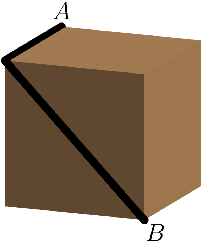
\includegraphics{intro-cube_0}
\end{minipage}
\smallbreak

\begin{minipage}[t]{0.51\linewidth}\vspace{0pt}
	\begin{enumerate}\setcounter{enumi}{1}
	  \item Two houses are to be connected to the electricity supply using a single connection.\par
	  How should we determine where to place the connection so as to minimize the required length of wire?\par
	  What information do you need in order to find the connection point?
	\end{enumerate}
\end{minipage}
\hfill
\begin{minipage}[t]{0.48\linewidth}\vspace{0pt}
	\flushright
	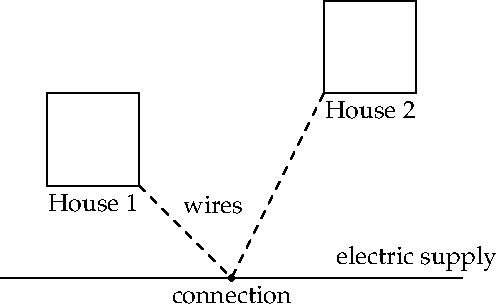
\includegraphics[scale=0.9]{intro-elec}
\end{minipage}
\medbreak

\footnotetext{%
	We are grateful to materials from UT Austin's UTeach program for suggesting several of the examples in this course including these motivational problems.%
}

Your goal shouldn't only be to find the right answer! Consider how you might discuss these problems with grade-school students of different ability levels. Why might calculus \emph{not} be a sensible approach? Are there any similarities between the two problems? Brainstorm some strategies\ldots

%Unfold for the first then straight line. Reflection helps for the second: make equal angle, so split the distance between the houses in same ratio as the distances from the houses to the wire (similar triangles).

\goodbreak



\section{Sets \&\ Functions}\label{chap:func}

\subsection{Basic Definitions}\label{sec:funcdef}

Consider how central functions are to mathematics, and how long you've been using them. How would you \emph{define} ``function'' to someone with limited mathematical knowledge? Would you use words like \emph{rule, assign, element, domain, vertical line test,} etc.? How helpful are these to your audience?

\begin{examples}{}{funcbasic}
	How would you explain the idea that the following do or do not represent functions?\vspace{-5pt}
	\begin{enumerate}\itemsep0pt
	  \item $y=x^2$
	  \item\label{ex:funcbasic2} Mon: fish,\quad Tue: pork,\quad Wed: fajitas,\quad Thur: carbonara,\quad Fri: pizza,\quad Sat: fish,\quad Sun: pizza
	  \item $(3,5)$, $(2,6)$, $(4,2)$, $(3,1)$.
	  \item $x^2=y^2$
	\end{enumerate}
\end{examples}

After considering the examples, perhaps you settle on a semi-formal definition:
\[
	\tcbhighmath{\text{A function $f$ is rule which assigns to each input $x$ exactly one output $f(x)$}}
\]
Is this a useful definition? In what ways is it imprecise? Does the imprecision matter?
\medbreak

Of course the answers to these questions depend on your audience! What ideas do you want to convey to your students and can you do so without overburdening and intimidating them? To begin working towards a more complete picture, consider what we might allow to be \emph{inputs} and \emph{outputs.} This requires a small amount of set notation.

\begin{defn}{}{}
	A \emph{set} $A$ is a collection of objects, or \emph{elements.}\footnotemark{} The notation $a\in A$ means that $a$ is an element of $A$, sometimes read `$a$ lies in $A$.' Sets are often written upper case and elements lower.\par
	\begin{minipage}[t]{0.75\linewidth}\vspace{-5pt}
		A set $B$ is a \emph{subset} of a set $A$, written $B\subseteq A$, if every element of $B$ is also an element of $A$: that is,
		\[
			b\in B\implies b\in A
		\]
		The picture illustrates sets $A,B$ and elements $a,b$ for which $B\subseteq A$, $a\in A$, $b\in B$ and $a\notin B$ ($a$ does not lie in $B$).
	\end{minipage}
	\hfill
	\begin{minipage}[t]{0.24\linewidth}\vspace{-6pt}
		\flushright
		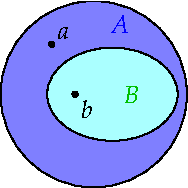
\includegraphics[scale=0.95]{functions-subset}
	\end{minipage}
\end{defn}

\footnotetext{%
	This is enough for our purposes, though a course in set theory will convince you that this definition has its own problems. Selection is always at work\ldots%
}


\begin{examples}{}{}
	\exstart Suppose the elements of a set $A$ are the numbers 1, 3, 5, 7 and 9. The simplest way to write this is using \emph{roster notation}: we list the elements (in any order) between braces
	\[
		A=\{1,3,5,7,9\}
	\]
	\begin{enumerate}\setcounter{enumi}{1}
	  \item[]Subsets are commonly expressed using \emph{set-builder notation}. %: $\{a\in A:\text{condition on $a$}\}$. 
	  For example, here is a subset of $A$:
	 	\[
	 		B=\{a\in A:2<a<8\} %\tag{the set of $a$ in $A$ such that $a$ lies strictly between 2 and 8}
	 	\]
	 	This is read, ``The set of $a$ in $A$ such that $a$ lies strictly between 2 and 8.'' In roster notation, $B=\{3,5,7\}$. Can you express $B$ in other ways using set-builder notation?
	 	
	  \goodbreak
  
	  \item We summarize several common sets of numbers using informal combinations of roster and set-builder notation, all of which should be familiar.
	  \begin{description}
			\item[Natural numbers] $\N=\{1,2,3,4,\ldots\}$. For instance, $5\in\N$ but $-3\not\in\N$.
			\item[Integers] $\Z=\{\ldots,-2,-1,0,1,2,3,\ldots\}$. For instance, $-4\in\Z$ but $\frac 45\not\in\Z$.
			\item[Rational numbers] (fractions) \ $\Q=\bigl\{\frac pq:p\in\Z,\ q\in\N\bigr\}$. For instance $-\frac 67\in\Q$; in this case $p=-6$ is an integer, and $q=7$ a natural number.
			\item[Real numbers] $\R$. For instance, $\sqrt 2\in\R$. A formal definition is difficult, though we often informally visualize $\R$ as a \emph{ruler}. \emph{Intervals} are particularly important subsets, e.g.,
			\[
				[-4,\pi)=\{x\in\R:-4\le x<\pi\}
			\]
			is a half-open interval.\smallbreak
			You should also be familiar with the \emph{Cartesian plane}: $\R^2=\{(x,y):x,y\in\R\}$. The notation $(3,4)\in\R^2$ here describes a \emph{point} in the plane with \emph{co-ordinates} $x=3$, $y=4$; don't confuse this with the \emph{interval} $(3,4)=\{x\in\R:3<x<4\}$ which is a subset of $\R$!
		\end{description}
		The subset relationships between these sets are in the order listed:
		\[
			\N\subseteq\Z\subseteq\Q\subseteq\R
		\]
		You should also have informally encountered the notion of \emph{irrationality}: for instance, $\sqrt 2$ and $\pi$ are real numbers but not rational numbers.
	\end{enumerate}
\end{examples}

\bigskip


The reason we need this language when discussing functions is that the inputs and outputs of a function are \emph{elements} of sets. Here is a \emph{very} formal definition of ``function.''

\begin{defn}{}{function}
	The \emph{Cartesian product} of sets $A,B$ is the set of \emph{ordered pairs}
	\[
		A\times B=\bigl\{(a,b):a\in A,b\in B\bigr\}
	\]
	A \emph{function} from $A$ to $B$ is a non-empty subset $f\subseteq A\times B$ which satisfies the \emph{vertical line test}
	\[
		\text{For each $a\in A$, there is a \emph{unique} $b\in B$ such that $(a,b)\in f$} \tag{$\ast$}
	\]
	Instead of writing $f\subseteq A\times B$ and $(a,b)\in f$, we use the more familiar notation
	\[
		f:A\to B\quad\text{and}\quad f(a)=b
	\]
	To a function $f:A\to B$ are associated three useful sets:
	\begin{itemize}\itemsep0pt
	  \item Domain: $\dom f=A$ is the set of \emph{inputs.}
	  \item Codomain: $\codom f=B$ is the set of \emph{possible outputs.}
	  \item Range: $\range f=\{b\in B:b=f(a)\text{ for some }a\in A\}$ is the set of \emph{realized outputs.}
	\end{itemize}
\end{defn}

This probably isn't the definition you should give to 10\th{} graders, or even to freshman calculus students! But what should you do? How much of this is helpful in a a given context?

\goodbreak


\begin{example*}{\ref{ex:funcbasic}.\ref{ex:funcbasic2} cont.}{}
	We revisit our food-based example in this formal setting. To properly view this as a function $f:A\to B$, we have to carefully label the constituent sets.
	\begin{gather*}
		A=\bigl\{\text{Mon, Tue, Wed, Thu, Fri}\bigr\},\qquad\qquad
		B=\bigl\{\text{carbonara, fajitas, fish, pizza, pork}\bigr\},\\[5pt]
		f=\bigl\{(\text{Mon,\ fish}),\ (\text{Tue,\ pork}),\ (\text{Wed,\ fajitas}), \ (\text{Thu,\ carbonara}),\\
		\qquad\qquad\qquad\qquad\qquad\qquad\qquad\qquad
		(\text{Fri,\ pizza}),\ (\text{Sat,\ fish}),\ (\text{Sun,\ pizza})\bigr\}
	\end{gather*}
	The domain $A$ should be clear, but we had to make a choice for the codomain $B$: in this case we chose it to equal to \emph{range.} Can you suggest a different choice for $B$? Try the other examples yourself.
\end{example*}


\boldsubsubsection{Representing Functions}

Functions can be represented in various ways. We illustrate a few in an example.

\begin{example}{}{introfunction}
	We consider the familiar \emph{formula/rule} $f(x)=x^2$ in several contexts.
	\begin{description}\itemsep8pt
	  \begin{minipage}[t]{0.71\linewidth}\vspace{-5pt}
	  	\item \emph{Table}\lstsp This presentation is most helpful when the domain is very small. The table shows the situation when $\dom f=\{-1,0,1,2,3\}$ and $\operatorname{range}f=\{0,1,4,9\}$
	  
	  	\item \emph{Arrows}\lstsp A pictorial arrow diagram might also be helpful when the domain is small.
	  
	  	\item \emph{Graph}\lstsp This is the set of ordered pairs $\bigl\{\bigl(x,f(x)\bigr):x\in\dom f\bigr\}$: in the context of the formal definition (\ref{defn:function}), \emph{the graph is the function!}\smallbreak
		 	For formulæ whose inputs and outputs are real numbers, two conventions are often observed:
		 	\begin{itemize}
		 	  \item The \textcolor{red}{domain} is \emph{implied} to be all real numbers for which the formula makes sense.
				\item The codomain is taken to be the set of real numbers.
			\end{itemize}
			If no other information is provided, we'd assume that the function defined by the formula $f(x)=x^2$ has both domain and codomain the entire set of real numbers: $f:\R\to\R$.
			\smallbreak
			
			The \textcolor{Brown}{range} of the function is the set of possible outputs, in this case
			\[
				\operatorname{range}f=\{x^2\in\R:x\in\R\}=[0,\infty)
			\]
			is the half-open interval of non-negative real numbers.
			\smallbreak
			
			For `calculus' functions like these, the vertical line test ($\ast$) really involves \textcolor{Green}{vertical lines}; every vertical line intersects the graph in precisely one point.
			\smallbreak
			In the picture, the \textcolor{orange}{dots} are the graph when the domain is the finite set $\{-1,0,1,2,3\}$ (as described in the table/arrow-diagram).
	  \end{minipage}
	  \hfill
	  \begin{minipage}[t]{0.28\linewidth}\vspace{0pt}
	  	\flushright
	  	$\begin{array}{@{}c|ccccc@{}}
				x&-1&0&1&2&3\\\hline
				f(x)&1&0&1&4&9
			\end{array}$
			\bigbreak
			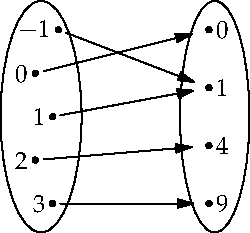
\includegraphics[scale=0.95]{functions-quad2}\bigbreak
			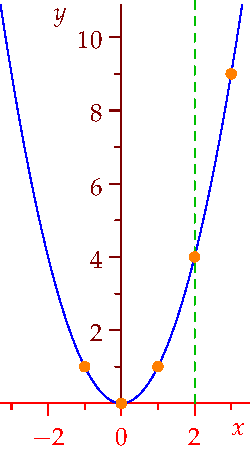
\includegraphics[scale=0.95]{functions-quad}
	  \end{minipage}
	\end{description}
\end{example}

Can you think of other ways to represent a function? How might you decide which to use?


\goodbreak


\begin{exercises}{}{}
	\exstart Let $d$ represent the cost in millions of dollars to produce $n$ cars, where $n$ is measured in 1000s. As clearly as you can, explain what is meant by $d(25)=431$. 

	\begin{enumerate}\setcounter{enumi}{1}
	  \item A movie theater seats 200 people. For any particular show, the amount of money the theater takes in is a function of the number of people $n$ in attendance. If a ticket costs \$25, describe the domain and range of the function using set notation.
	  
	  
		\item\label{exs:templinear} Temperature readings $T$ were recorded every two hours from midnight to noon. Time $t$ was measured in hours from midnight.
	  \[
	  	\begin{array}{l|ccccccc}
	  		t&0&2&4&6&8&10&12\\\hline
	  		T\ (^\circ\mathrm{F})&82&75&74&75&84&90&93
	  	\end{array}
	  \]
	  \begin{enumerate}
	    \item Plot the readings and use them to sketch a rough graph of $T$ as a function of $t$.
	    \item Use your graph to estimate the temperature at 10:30\AM
	  \end{enumerate}
	  
	  
	  \item State parts 1, 3 and 4 of Example \ref{ex:funcbasic} using the formal language of Definition \ref{defn:function}. If you have a function, state the domain and range and explain how you know you have a function. If you don't have a function, explain why not.
	  \par
	  (\emph{Since insufficient information is provided, there is no single correct answer!})
	  
	  
	  \item\begin{enumerate}
	    \item Let $A=\{1,3,5,7,9\}$. Explain in words what is meant by the set
	    \[
	    	B=\{x\in A:x^2>10\}
	    \]
	    and state $B$ in roster notation.
	    \item Find the set $C=\{x\in\N:(x-1)^2<16\}$ in roster notation.
	    \item Find the Cartesian product $B\times C$ in roster notation. Is it the same as $C\times B$?
	  \end{enumerate}
	  
	  
	  \item Suppose that $f:\{-2,-1,0,1,2\}\to\R$ is defined by the formula $f(x)=x^3-4x+1$.\par
	  Describe $f$ using a table, an arrow diagram and a graph.
	  
	  
	  \item Find the implied domain and range for the functions defined by each rule:
	  \begin{enumerate}
	    \item $f(x)=\frac{x^2-4}{x-2}$\qquad\qquad
	    (b) \ $g(x)=\sqrt{x^2-16x}$\qquad\qquad
	    (c) \ $h(x)=\frac 1x\sqrt{4x-x^2}$
	  \end{enumerate}
	  (\emph{What is the largest set of real numbers for which the formula makes sense}?)
	  
	  
	  \item You ask your students to determine the range of the function $f$ defined by the rule $f(x)=x^2$ with domain the interval $[-5,2]$. You obtain various responses, including $[25,4]$, $[4,25]$, and $[-25,4]$. What is going wrong? What is the correct answer, and how would you explain it to your students?\par
	  More generally, if $\dom f=[a,b]$ (where $a\le b$), what is $\range f$?
	  
	  
	  \item The unit circle is often represented by the implicit equation $x^2+y^2=1$.
	  \begin{enumerate}
	    \item Draw the circle and explain why the full circle isn't the graph of a function.
	    \item Describe \emph{two} functions $f:[-1,1]\to\R$ and $g:[-1,1]\to\R$ whose graphs together comprise the circle. What are the ranges of each function?
	  \end{enumerate}
	  
	\end{enumerate}
\end{exercises}



\clearpage



\subsection{Linear Polynomials}

Perhaps the simplest functions are the \emph{linear polynomials}, whose graphs are straight lines,
\[
	y=f(x)=mx+c\quad\text{where $m,c$ are constants} \tag{$\ast$}
\]
Linear polynomials make very simple models: increase the input by $\Delta x$ and the output changes by $\Delta y=m\Delta x$ \emph{regardless} of the starting value $x$. Given experimental data or a physical situation relating two quantities $x$ and $y$, a \emph{linear model} is an linear polynomial ($\ast$) relating these variables. In practice, models are \emph{approximations} to the real-world data. Later in the course we'll consider what should be meant by, and how to find, a `good' linear model for approximately linear data.\smallbreak

Some of your earliest forays into algebra likely involved finding equations of straight lines.

\begin{example}{}{mxplusc}
	Find the equation of the \textcolor{blue}{straight line} through the points $A=(1,3)$ and $B=(4,1)$.
	\par
	\begin{minipage}[t]{0.64\linewidth}\vspace{-5pt}
		Suppose the polynomial is $y=mx+c$. Since both $A$ and $B$ satisfy this equation, we start by substituting both points into the equation to find two relationships between $m$ and $c$
		\[
			\begin{cases}
				3=m+c\\
				1=4m+c
			\end{cases}
		\]
		This is a system of two linear equations in two unknowns ($m,c$). By now you should know several ways to solve such, but consider what might be easiest for a grade-school student\ldots
	\end{minipage}
	\hfill
	\begin{minipage}[t]{0.35\linewidth}\vspace{0pt}
		\flushright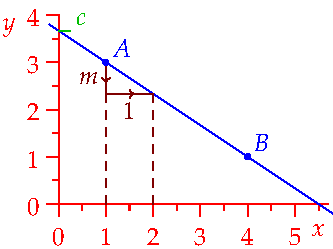
\includegraphics{line-line}
	\end{minipage}
	\medbreak 
	Regardless of how you phrase it (solve one equation for $c$ and substitute into the other, subtract one question from the other, etc.), we obtain
	\[
		-2=3m\implies m=-\frac 23\implies c=3-m=\frac{11}3
	\]
	whence the required polynomial is $y=\frac 13(11-2x)$.\smallbreak
	As the picture suggests, the \emph{\textcolor{Brown}{gradient/slope} $m$} represents how far one climbs/falls on travelling one unit to the right.	The \textcolor{Green}{\emph{$y$-intercept} $c$} is the intersection of the graph with the vertical axis.
\end{example}

The above process works for any two points $A=(x_0,y_0)$ and $B=(x_1,y_1)$ provided $x_0\neq x_1$: is it clear why this should be the case? The details are in Exercise \ref{exs:lineparam}. You might feel that such a problem is too abstract for your students, that such a `proof' might be too intimidating. Indeed it might be counterproductive for some students, but consider several counterpoints:
\begin{itemize}
  \item Once a student has developed comfort with concrete examples as above, Exercise \ref{exs:lineparam} helps summarize and unify what they've learned. A general/abstract discussion helps build confidence by convincing a student that any such problem can be solved the same way.
  \item The most helpful elementary proofs are those which essentially replicate an example abstractly. Exercise \ref{exs:lineparam} is not some abstract existence proof---it involves no trickery---it simply \emph{reinforces} the core technique by applying it in the most general situation.
  \item Helping and encouraging students to think abstractly is one of the overarching learning outcomes of all mathematics. You might get push-back, but it's part of the job\ldots
\end{itemize}


\goodbreak


\begin{example}{}{beakers}
	Often the challenge of modeling lies in converting a word problem into algebra---don't underestimate how hard students find this! Here is a simple, though disguised, straight line model.\smallbreak
	Beaker A contains a 300\,ml solution of 2\% acid. Beaker B contains 400\,ml of acid of unknown concentration. The beakers are mixed together to produce an acid with concentration 6\%. What was the concentration in beaker B?\smallbreak
	\emph{Given your mathematical experience}, it should seem natural to denote the unknown concentration (beaker B) by $x$. After mixing, we have a 700\,ml solution containing $300\times\frac 2{100}+400x$\,ml of pure acid, whence its concentration is a linear polynomial function of $x$:
	\[
	 C(x)=\frac{6+400x}{700}
	\]
	The problem is now easily solved: $C(x)=\frac 6{100}\Longleftrightarrow x=\frac 9{100}=9\%$.
\end{example}



\boldinline{Parametrized Lines}\phantomsection\label{pg:paramline}

Straight lines admit an alternative visualization. Imagine placing a \emph{ruler} so that its zero point is at the origin $O=(0,0)$ and the ``1" lies at a point $C=(c_1,c_2)$. If $t$ (a real number) is the measure on the ruler, then the points on the line have co-ordinates
\[
	tC=(tc_1,tc_2) \tag{$\ast$}
\]

\begin{minipage}[t]{0.65\linewidth}\vspace{-8pt}
	To describe the line through points $A$ and $B$, place a ruler so that \textcolor{Green}{0} corresponds to $A$ and \textcolor{Green}{1} to $B$. Now \textcolor{Brown}{slide} the ruler so that $A$ moves to the origin $O$: this amounts to \emph{subtracting} the co-ordinates of $A$ from all points on the line. We obtain a parallel line through the origin, with $B$ transformed to the point $C=B-A$. Putting this together with ($\ast$) results in a parametrized description of the line:
	\[
		(x,y) =A+\textcolor{Green}{t}C
		=A+\textcolor{Green}{t}(B-A)
		=(1-\textcolor{Green}{t})A+\textcolor{Green}{t}B
	\]
	\end{minipage}
	\hfill
	\begin{minipage}[t]{0.34\linewidth}\vspace{0pt}
		\flushright
		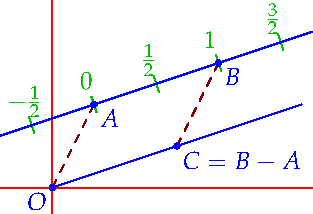
\includegraphics{line-line2}
	\end{minipage}\bigbreak

%The points corresponding to various values of $t$ are \textcolor{Green}{marked}.\medbreak

Contrast the parametrized description of a line with the linear polynomial approach: for instance, one challenge is that a line may be parametrized using infinitely many distinct rulers (choose \emph{any} two points on the line!), whereas the linear polynomial description is unique. Does the parametrized approach have any advantages? Which description is easier to understand or to work with? Which fits better with your intuitive understanding of \emph{line}? Which might cause a grade-school student the greater challenge?\smallbreak

In the Exercises we make sure that the two descriptions of a line correspond. The discussion is little more than the generalization of an example.

\begin{example}{}{}
	The line through points $A=(3,6)$ and $B=(-1,4)$ may be parametrized by
	\[
		(x,y)=(1-t)(3,6)+t(-1,4)=\bigl(3-4t,6-2t\bigr)
	\]
	To convert this to a linear polynomial, first solve for $t$ in terms of $x$,
	\[
		x=3-4t\implies t=\frac 14(3-x)
	\]
	before substituting into our expression for $y$:
	\[
		y=6-2t=6-\frac 24(3-x) =\frac 12x-\frac 92
	\]
\end{example}



\goodbreak



\begin{exercises}{}{}
	\exstart The cost of gasoline is \$4.20 per gallon on January 1\st{} and \$4.90 on March 1\st. State a \emph{linear} function/model for the cost of gasoline as a function of time.


	\begin{enumerate}\setcounter{enumi}{1}
	  \item You have a choice of three different cell-phone plans.
	  \begin{enumerate}
	    \item No monthly charge and 10\textcent{} per minute for all calls.
	    \item \$10 per month and 5\textcent{} per minute for all calls.
	    \item \$30 per month, regardless of how many calls you make.
	  \end{enumerate}
	  How should you determine which plan to purchase?
	  
	  
	  \item Revisit Exercise \ref*{sec:funcdef}.\ref{exs:templinear}. Find an approximate linear model $T(t)=mt+c$ for this data.\par
	  (\emph{There is no perfect answer})
	  
	  
	  \item Revisit the beakers problem (Example \ref{ex:beakers}). This time suppose we know that the concentration in beaker B is 9\%. How much from beaker B should we pour into beaker A to obtain an acid with concentration 5\%? Would you consider this a linear polynomial problem? Why/why not?
    
    
    \item\label{exs:lineparam}
    Suppose points $A=(x_0,y_0)$ and $B=(x_1,y_1)$ are given. 
    \begin{enumerate}
      \item If $x_1\neq x_0$, use the method of Example \ref{ex:mxplusc} to find the equation $y=mx+c$ of the line through these points.
      
      \item Now use the parametrized approach where $A$ corresponds to 0 and $B$ to 1. If, in addition, $x_1\neq x_0$, make things match up with your answer to part (a).\par
      What parametrization do you get if $A=(0,c)$ and $B=(1,m+c)$?
	  
			\item Part (a) provides an \emph{algebraic} justification of the claim made on page \pageref{pg:paramline}, that the linear polynomial description of a line is unique (`\emph{the} equation'). How might you help a student believe this claim if the algebra is unconvincing or too intimidating?\par
			(\emph{Think about Example \ref{ex:mxplusc}})
    \end{enumerate}
        
    
    \item A straight line is sometimes described as the set of points $(x,y)\in\R^2$ satisfying an equation of the form
    \[
    	ax+by=c
    \]
    for some constants $a,b,c$ where $a,b$ are not both zero. How does this approach differ from our use of linear polynomials?
    
    
    \item Throughout mathematics (particularly within \emph{linear algebra}), a function $f:\R\to\R$ is said to be \emph{linear} if it satisfies the condition
    \[
    	\text{For all }\lambda,x\in\R,\quad f(\lambda x)=\lambda f(x)
    \]
    Is this the same thing as a linear polynomial? Explain.
   
  \end{enumerate}
\end{exercises}



\clearpage



\subsection{Quadratic Polynomials}

Quadratic polynomials are functions of the form $y=f(x)=ax^2+bx+c$ where $a\neq 0$. The simplest is $y=x^2$, the standard parabola opening upwards. Here are some commonly encountered activities:
\begin{enumerate}\itemsep0pt
  \item Find the \emph{roots/zeros} of $f$, the solutions $x$ to the equation $f(x)=0$.
  \item Sketch the \emph{graph} of the function $f$.
  \item Use quadratic functions to model a real-world problem.
\end{enumerate}

You likely know two methods for finding zeros: factorizing and the quadratic formula, each of which has its problems. With experience it is easy to spot that 
\[
	x^2+2x-15=(x-3)(x+5)=0\iff x=3\text{ or }x=-5
\]
though the required creativity can make this difficult, particularly when coefficients are large. Students often prefer the quadratic formula since it always works, though at the cost of some intimidating algebra. We'll think about factorization shortly. First, we see how \emph{completing the square} lies behind both the quadratic formula and the standard approach to graphing quadratic functions.

\begin{example}{}{quadraticeasy}
	Describe/graph the parabola $y=-3x^2+12x+4$.\par
	\begin{minipage}[t]{0.62\linewidth}\vspace{-5pt}
		Pay attention to the $x$ terms; $-3x^2+12x=-3(x^2-\textcolor{red}{4}x)$. Now
		\[
			-3(x-\textcolor{red}{2})^2=-3(x^2-\textcolor{red}{4}x+4)=-3x^2+12x-12
		\]
		gives most of what we want: note how we \emph{divided the \textcolor{red}{$x$-coefficient} by two.} To finish, just tidy everything up,
		\[
			y=(-3x^2+12x-12)+16=-3(x-2)^2+16
		\]
	\end{minipage}
	\hfill
	\begin{minipage}[t]{0.27\linewidth}\vspace{-15pt}
		\flushright
		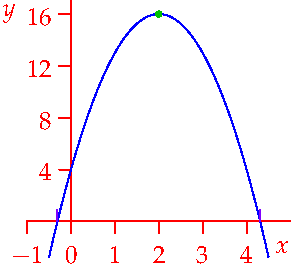
\includegraphics[scale=0.9]{poly-quad2}
	\end{minipage}\medbreak
	The parabola therefore opens downwards ($-3<0$) with its \textcolor{Green}{apex} (maximum) at $(x,y)=(2,16)$.
\end{example}

This is easy, if intimidating, to repeat in general:
\begin{align*}
	ax^2+bx+c&=a\left(x^2+\frac ba x\right)+c =a\left[\left(x+\frac b{2a}\right)^2-\frac{b^2}{4a^2}\right]+c\\
	&=a\left(x+\frac b{2a}\right)^2-\frac{b^2-4ac}{4a} \qquad\qquad\qquad\qquad(\ast)
\end{align*}
\begin{minipage}[t]{0.6\linewidth}\vspace{0pt}
	The graph is that of the standard parabola which has been:
	\begin{enumerate}\itemsep0pt
	  \item Vertically scaled by $a$;
	  \item Shifted horizontally by $-\frac b{2a}$;
	  \item Shifted vertically by $\frac{4ac-b^2}{4a}$
	\end{enumerate}
	By solving ($\ast$) for $x$, we see that completing the square yields the \emph{quadratic formula.}
\end{minipage}
\hfill
\begin{minipage}[t]{0.39\linewidth}\vspace{-60pt}
	\flushright
	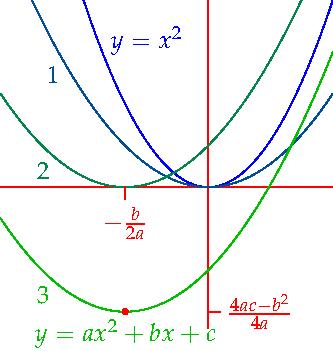
\includegraphics[scale=0.9]{poly-quad}
\end{minipage}

\begin{thm}{}{}
	If $a\neq 0$, then $ax^2+bx+c=0\iff x=\dfrac{-b\pm\sqrt{b^2-4ac}}{2a}$
\end{thm}


\goodbreak


\begin{example*}{\ref{ex:quadraticeasy} cont}{}
	Our analysis suggests two methods for finding the \textcolor{purple}{roots}.
	\begin{enumerate}
	  \item Quadratic formula: with $a=-3$, $b=12$, $c=4$, we have
	  \[
	  	x=\dfrac{-12\pm\sqrt{12^2-4(-3)\cdot 4}}{2(-3)} =\dfrac{-12\pm 4\sqrt{3^2+3}}{-6} =2\pm\dfrac{\sqrt{12}}{3} =2\pm\dfrac{2\sqrt{3}}{3}
	  \]
	  While it is always tempting to jump for a formula, it often leads to difficult surd expressions. We simplified by noticing the common factor of $4^2$ inside the square root. Without this, we'd be faced with $\sqrt{144+48}=\sqrt{192}$.
	  \item Use the fact that we've already completed the square:
	  \[
	  	-3(x-2)^2+16=0\iff (x-2)^2=\frac{16}3\iff x=2\pm\frac 4{\sqrt 3}
	  \]
	  In many cases it is simpler to complete the square than to use the quadratic formula---remember that they are equivalent!
	\end{enumerate}
\end{example*}


Polynomials are often employed in modelling due to their simplicity and ease of evaluation. As you saw in calculus, the motion of a falling body, or of any projectile can be modelled using quadratic polynomials, an observation going back to at least to Galileo in the early 1600s: the distance travelled by a falling body is proportional to the \emph{square} of the time taken $y(t)-y(0)\propto t^2$.

\begin{example}{}{quadseqgraph}
	A body is dropped from a height of 125 meters, taking exactly 5 seconds to reach the ground. Its height at time $t$ seconds is given by $y(t)=125-5t^2$\,m.\smallbreak
	\begin{minipage}[t]{0.68\linewidth}\vspace{-8pt}
	This certainly fits Galileo's observation: $y(t)-y(0)=-5t^2$ is indeed proportional to $t^2$.\smallbreak
	Over each interval of 1\,s, we may ask how far the body falls; we summarize in a table.
	\[
		\begin{array}{c|ccccccccccc}
			t&0&&1&&2&&3&&4&&5\\\hline
			y(t)&125&&120&&105&&80&&45&&0\\\hline
			y(t)-y(0)&0&&-5&&-20&&-45&&-80&&-125\\\hline
			\Delta y&&\makebox[0pt][c]{$-5$}&&\makebox[0pt][c]{$-15$}&&\makebox[0pt][c]{$-25$}&&\makebox[0pt][c]{$-35$}&&\makebox[0pt][c]{$-45$}
		\end{array}
	\]
	\end{minipage}
	\hfill
	\begin{minipage}[t]{0.29\linewidth}\vspace{-25pt}
		\flushright
		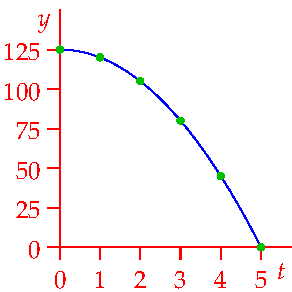
\includegraphics{poly-quad5}
	\end{minipage}\medbreak
	Since each interval has duration 1\,s, each $\Delta y$ is the \emph{average speed} of the falling body over that interval.
\end{example}

You'll have seen problems like this in calculus; likely you want to \emph{differentiate} to find the \emph{velocity} $y(t)=-10t$\,m/s and \emph{acceleration} $y''(t)=-10$\,m/s$^2$. However, historically and in introductory calculus, it is problems like these that \emph{motivate the definition} of the derivative.\footnote{The last line of the table really does suggest that speed is a linear function!}\par
Armed with calculus, Galileo's observation is that the height $y(t)$ solves the differential equation
\[
	\diff[^2y]{t^2}=-g
\]
where $g$ is the constant acceleration due to gravity; approximately 32\,ft/s$^2$ or 10\,m/s$^2$. Unless you are explicitly teaching calculus or Newtonian physics, this is probably a bad place to start! 



\begin{example}[lower separated=false, sidebyside, sidebyside align=top seam, sidebyside gap=0pt, righthand width=0.3\linewidth]{}{frisbee}
	Your frisbee is stuck 15\,m up a tree. Standing 10\,m from the base, you throw a ball with the intent of knocking the frisbee out of the tree.\smallbreak
	The standard approach to modelling such problems involves considering the horizontal and vertical motions separately.
	\begin{quote}
		\emph{Horizontal}\lstsp $x(t)=pt+q$ is a \emph{linear function} of time.\smallbreak
		\emph{Vertical}\lstsp $y(t)=-10t^2+rt+s$ is a \emph{quadratic function} of time.
	\end{quote}
	Substituting for $t$ yields a quadratic function for the \textcolor{blue}{trajectory}
	\[
		y(x)=ax^2+bx+c
	\]
	We'll leave the details of the solution to Exercise \ref{exs:frisbee}. For the present, consider why there are \emph{multiple answers}; can you explain why \emph{without} explicitly solving the problem?
	\tcblower
	\flushright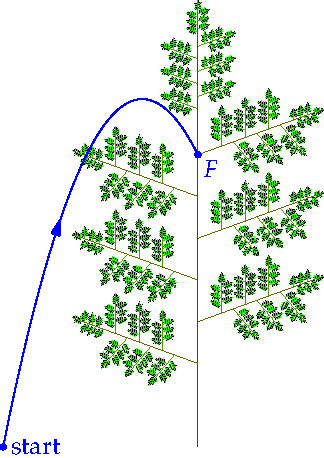
\includegraphics[scale=0.88]{tree1}
\end{example}


\begin{exercises}{}{}
	\exstart Complete the square for each quadratic function, use it to find the range and to graph the function.
	\begin{enumerate}\setcounter{enumi}{1}  
	  \item[]\begin{enumerate}
	    \item $f(x)=x^2-6x+5$ %$(x-3)^2-4$
	    \item $f(x)=-x^2+x+1$ %$-(x-\frac 12)^2+\frac 54$
	    \item $f(x)=-3x^2+8x+5$ %$3(x+\frac 43)^2-\frac 13$
	  \end{enumerate}
	  %For part (a), also find two intervals $(-\infty,k]$ and $[k,\infty)$ (same $k$!) on which $f$ is invertible. For each interval, compute the inverse function $f^{-1}$.
	  
	  
	  \item For the quadratic function $y=2x^2-5x+7$, produce a table for $x\in\{0,1,2,3,4,5,6\}$ similarly to that in Example \ref{ex:quadseqgraph}. What do you observe about $\Delta y$?
	  
	  
		\item\begin{enumerate}
		  \item Find the equations of all quadratic polynomial functions which pass through the points $(1,3)$ and $(2,4)$.
			\item More generally, if $P=(a,b)$ and $Q=(c,d)$ are given, where $c\neq a$, find all quadratic functions whose graphs contain $P$ and $Q$.
		\end{enumerate}
	  
	  \item\label{exs:frisbee} Consider the frisbee/tree problem (Example \ref{ex:frisbee}).
	  \begin{enumerate}
	    \item Assume that you're standing at the origin and the frisbee is at the point $(10,15)$. Find all trajectories.
	    \item (Hard)\lstsp Find a formula linking the initial speed and gradient of the parabola (the initial speed and direction in which you throw the ball).
	    \begin{enumerate}
				\item If you throw the ball in such a way that the initial \emph{vertical} speed of the ball is twice its \emph{horizontal} speed, find how fast you have to throw the ball in order to hit the frisbee.
	      \item What is the \emph{minimum} speed at which you could throw the ball if you want to dislodge the frisbee?
	    \end{enumerate}
	    (\emph{Hint: You'll need some calculus! In the language of the original problem, the initial slope is $m=\frac rp$ and speed $v=\sqrt{p^2+r^2}$; why?})
		\end{enumerate}

	\end{enumerate}
\end{exercises}

\clearpage



\subsection{Polynomials, Factorization \& the Rational Roots Theorem}

Recall our simple example of factorization in the previous section
\[
	x^2+2x-15=(x-3)(x+5)=0\iff x=3\text{ or }x=-5
\]
That this approach provides \emph{all} roots depends on several familiar algebraic facts:
\begin{enumerate}
  \item Factor Theorem: $f(c)=0\iff x-c$ is a \emph{factor} of $f(x)$.
  \item No zero-divisors: $pq=0\iff p=0$ or $q=0$. 
  \item A quadratic has \emph{at most two} distinct roots.
\end{enumerate}
We'll examine this more closely at the end of this section. For students first learning factorization, it isn't the \emph{why} that's the challenge, it's the \emph{how.} Multiplying out $(x-3)(x+5)$ is mechanical, but factorizing requires some creativity; we can't really factor without somehow knowing that 3 and $-5$ are roots! Beyond making a lucky guess, how do we go about this? 

\begin{example}{}{ratroots1}
	Let's re-examine $f(x)=x^2+2x-15=0$ in a couple of stages.
	\begin{description}
		\item[\normalfont\emph{Integer solutions}] The simplest type of root would be an \emph{integer} $n$. If $f(n)=0$, observe that
		\begin{align*}
			n^2+2n-15=0&\implies n(n+2)=15\implies \text{15 is divisible by $n$}\\
			&\implies n=\pm 1,\pm 3,\pm 5,\pm 15
		\end{align*}
		There are only \emph{eight possible candidates.} It doesn't take long to test all of them:
		\[
			\begin{array}{c|cccccccc}
				n&1&-1&\textcolor{red}{3}&-3&5&\textcolor{red}{-5}&15&-15\\\hline
				f(n)&-12&-17&\textcolor{red}{0}&-12&20&\textcolor{red}{0}&240&180
			\end{array}
		\]
		The two integer solutions are therefore $x=3$ and $x=-5$.
		\item[\normalfont\emph{Rational Solutions}] If you believe that a quadratic polynomial has \emph{at most} two solutions, then you're done. The next simplest possibility, however, is that a solution be a \emph{rational number} $x=\frac pq$ where we may assume this is in \emph{simplest terms}.\footnotemark{} Substituting into the polynomial, we see that
		\[
			\frac{p^2}{q^2}+2\frac pq-15=0\iff p^2+2pq-15q^2=0
		\]
		Remembering that $p,q$ are \emph{integers,} we rearrange this equation in two ways:
		\begin{description}
		  \item[$\textcolor{blue}{p}(p+2q)=15q^2$]\lstsp Since the \textcolor{blue}{left side} is a multiple of $p$, so also is the \emph{right.} Since $p,q$ have no common factors, it follows that $p$ divides into 15 (15 is a multiple of $p$).
		  \item[$p^2=\textcolor{red}{q}(15q-2p)$]\lstsp Since the \textcolor{red}{right side} is a multiple of $q$, so also is the \emph{left.} Since $p,q$ have no common factors, we conclude that $q=1$.
		\end{description}
		The upshot is that the only rational solutions to $f(x)=0$ are the two \emph{integers} we've already found!
	\end{description}
\end{example}

\footnotetext{I.e., $p\in\Z$ and $q\in\N$ have no common factors: $\gcd(p,q)=1$.}

\goodbreak

\begin{defn}{}{}
	A \emph{degree $n$ polynomial} is any function of the form
	\[
		f(x)=a_nx^n+a_{n-1}x^{n-1}+\cdots+a_1x+a_0
	\]
	where the \emph{coefficients} $a_k$ are constants with $a_n\neq 0$.
\end{defn}

A quadratic polynomial has degree 2 and a linear polynomial $mx+c$ degree one\footnote{A non-zero constant polynomial has degree zero. Convention is for the \emph{zero polynomial} $y\equiv 0$ to have degree $-\infty$, so that the theorem $\operatorname{deg} fg=\operatorname{deg} f+\operatorname{deg} g$ holds for all polynomials.} (if $m\neq 0$).\smallbreak

Our analysis in Example \ref{ex:ratroots1} is easily generalized in a famous result.

\begin{thm}{Rational Roots}{}
	Suppose $f(x)=\textcolor{blue}{a_n}x^n+\cdots+\textcolor{red}{a_0}$ has \emph{integer} coefficients where $a_n$ and $a_0$ are non-zero. If $x=\frac pq$ is a rational root in simplest terms, then $\textcolor{blue}{q}$ divides into $\textcolor{blue}{a_n}$ and $\textcolor{red}{p}$ divides into $\textcolor{red}{a_0}$.
\end{thm}

\begin{proof}
	Substitute into the function and multiply by $q^n$ to obtain an equation where everything is an \emph{integer}\vspace{-13pt}
	\[
		\underbrace{a_np^n+a_{n-1}p^{n-1}q+\cdots+a_1pq^{n-1}}_{\text{divisible by $\textcolor{red}{p}$}} \hspace{-129pt} \overbrace{\phantom{a_{n-1}p^{n-1}q+\cdots+a_1pq^{n-1}}+a_0q^n}^{\text{divisible by $\textcolor{blue}{q}$}}=0
	\]
	By considering the braced terms and recalling that $p,q$ have no common factors, we conclude that $a_n$ is divisible by $q$ and $a_0$ by $p$.
\end{proof}


\begin{examples}{}{}
	\exstart If $x=\frac pq$ is a rational root in lowest terms of $f(x)=2x^2-x-3$, then $q=1$ or 2 and $p=\pm 1$ or $\pm 3$. The possibilities are therefore
	\[
		x\in\bigl\{\pm 1,\pm 3,\pm\tfrac 12,\pm\tfrac 32\bigr\}
	\]
	all of which are easily checked:
	\[
		\def\arraystretch{1.1}
		\begin{array}{c|cccccccc}
			x&1&\textcolor{red}{-1}&3&-3&\frac 12&-\frac 12&\textcolor{red}{\frac 32}&-\frac 32\\\hline
			f(x)&-2&\textcolor{red}{0}&12&18&-3&-2&\textcolor{red}{0}&3
		\end{array}
	\]
	The two roots are indicated and the polynomial can be factorized $f(x)=(2x-3)(x+1)$.
	\begin{enumerate}\setcounter{enumi}{1}
	  \item If the cubic polynomial $f(x)=x^3-2x^2+5$ had any rational roots, the only possibilities would be $\pm 1, \pm 5$. However, none of these work,
	  \[
	  	f(1)=4,\quad f(-1)=2,\quad f(5)=80,\quad f(-5)=-170
	  \]
	  whence $f(x)=0$ has no rational roots.
	\end{enumerate}
\end{examples}

Unless there are very few candidates, it can be time-consuming to check them all by hand. Moreover, unless you find $n$ distinct rational solutions, you still don't know that you've found everything. The rational roots theorem is therefore typically used together with factorization; it really just gives you some options for where to start. This still isn't easy, as the next example shows.
\goodbreak

\begin{example}{}{factoreasy}
	Consider the cubic function $f(x)=x^3-x^2-7x+10$. The rational roots theorem gives us eight candidates for rational roots: $x=\pm 1,\pm 2,\pm 5,\pm 10$. It is not difficult to check the first few of these in your head, for instance,
	\[
		f(2)=8-4-14+10=0
	\]
	By the factor theorem, $x-2$ must be a factor of $f(x)$. The factorization can be performed in various ways. Here are three options, though all are essentially versions of the same process.
	\begin{description}
	\item[\normalfont\emph{Long/synthetic division}]\lstsp You should have practiced this in high-school.
  \[
  	\polylongdiv{x^3-x^2-7x+10}{x-2} \implies x^3-x^2-7x+10=(x-2)(x^2+x-5)
  \]
  \item[\normalfont\emph{Multiply out and solve}]\lstsp We know that $f(x)=(x-2)q(x)$ where $q(x)$ is some quadratic polynomial. Thus let $q(x)=ax^2+bx+c$ and multiply out:
  \[
  	x^3-x^2-7x+10=(x-2)(ax^2+bx+c) =ax^3+(b-2a)x^2+(c-2b)x-2c
  \]
  Equating coefficients, we obtain the same factorization as before,
  \[
  	a=1,\quad b=-1+2a=1,\quad c=\frac{10}{-2}=-5
  \]
  \item[\normalfont\emph{Term-by-term factorization}]\lstsp With practice you can factorize in one line with no working!
  \begin{enumeratea}
    \item To create $\textcolor{red}{x^3}$, the first term of the quadratic factor must be $\textcolor{red}{x^2}$ 
    \[
    	\textcolor{red}{x^3}\textcolor{blue}{\,-\,x^2}\textcolor{Green}{\,-\,7x}\textcolor{purple}{\,+\,10}=(x-2)(\textcolor{red}{x^2}\,+\cdots)=\textcolor{red}{x^3}\,-2x^2+\cdots
    \]
    \item To correct the \textcolor{blue}{$x^2$} term, add $\textcolor{Green}{x}$ (i.e., $\textcolor{Green}{x^2}-2x^2=\textcolor{blue}{-x^2}$):
    \[
    	(x-2)(x^2+\,\textcolor{Green}{x}\,+\cdots)=\textcolor{red}{x^3}\textcolor{blue}{\,-\,x^2}\,\textcolor{Green}{-\,2x}+\cdots
    \]
    \item To correct the \textcolor{Green}{$x$} term, subtract $\textcolor{purple}{5}$:
    \[
    	(x-2)(x^2+x-\textcolor{purple}{\,5})=\textcolor{red}{x^3}\textcolor{blue}{\,-\,x^2}\,\textcolor{Green}{-\,7x}\textcolor{purple}{\,+\,10}
    \]
    \item Since the last term $\textcolor{purple}{10}$ is correct, the factorization worked!
	\end{enumeratea}
\end{description}
	
	You might have seen other approaches involving arranging the coefficients in a table. Regardless, the calculations required to complete these methods are exactly those seen above; all these methods are versions of the same thing.
\end{example}

\goodbreak



\boldsubsubsection{Why Does Factorization Work?}

The theory of factorization relies on some algebra. Here is a \emph{brief} treatment.

\begin{thm}{Factor Theorem}{}
	Suppose $f(x)$ is a degree $n$ polynomial. Then:
	\begin{enumerate}
	  \item A value $c$ is a root if and only if $f(x)=(x-c)q(x)$ for some (degree $n-1$) polynomial $q(x)$.
	  \item The polynomial has \emph{at most} $n$ distinct roots.
	\end{enumerate} 
\end{thm}

\begin{proof}
	\begin{enumerate}
	  \item ($\Leftarrow$)\lstsp This is essentially trivial: $f(x)=(x-c)q(x)\implies f(c)=(c-c)q(c)=0$.\smallbreak
		($\Rightarrow$)\lstsp This relies on the \emph{division algorithm for polynomials}: if $f,g$ are polynomials, then there are unique polynomials $q,r$ with\footnotemark{}
	% \footnote{Let $S=\{f(x)-g(x)q(x):q(x)\in\R[x]\}$. If $0\in S$  stop; $g$ divides $f$. Otherwise, let $k=\min S$ (exists by well-ordering) and let $r(x)=f(x)-g(x)q(x)=a_kx^k+\cdots$ have degree $k$. If $g(x)=b_jx^j+\cdots$ has degree $j\le k$, observe that
	% \[f(x)-g(x)\bigl(q(x)+\tfrac{a_k}{b_j}x^{k-j}\bigr)=r(x)-a_kx^k-\cdots\]
	% has degree $<k=\deg r$: contradiction. Thus $\deg r<\deg g$.\smallbreak
	% For uniqueness, suppose had two candidates $r_1,r_2$, then
	% \[r_1-r_2=g(q_2-q_1)\]
	% But $\deg(r_1-r_2)<\deg g$ and $\deg(g(q_2-q_1))\ge \deg g$ is a contradiction unless $q_1=q_2$ and both sides are zero.}
		\[
			f(x)=g(x)q(x)+r(x)\quad \text{and}\quad \deg r<\deg g
		\]
		In the special case where $g(x)=x-c$ is linear, then $r(x)$ must be a constant and so
		\[
			f(x)=(x-c)q(x)+f(c)
		\]
		\item Suppose $c_1,\ldots,c_n$ are distinct real roots. By part 1, $f(x)=(x-c_1)q_1(x)$. Since
		\[
			0=f(c_2)=(c_2-c_1)q_1(c_2)\implies q_1(c_2)=0
		\]
		we may factor $x-c_2$ from $q_1(x)$ to obtain
		\[
			f(x)=(x-c_1)(x-c_2)q_2(x),\qquad \deg q_2=n-2
		\]
		Repeat this process to factor out all $n$ linear polynomials $x-c_k$:
		\[
			f(x)=(x-c_1)\cdots(x-c_n)q_n,\qquad \deg q_n=n-n=0
		\]
		It follows that $q_n\neq 0$ is \emph{constant.} Plainly $f(c)=(c-c_1)\cdots(c-c_n)q_n=0\Longrightarrow c=c_j$ for some $j$, so there are no other roots.\qedhere
	\end{enumerate}
\end{proof}

\footnotetext{For a given example, $q,r$ may be found by synthetic division. This is similar (and may be demonstrated similarly) to the more familiar division algorithm for integers: if $m,n$ are integers, then there are unique integers $q,r$ for which
\[
	m=qn+r\ \text{ and }\ 0\le r<\nm n
\]
In elementary school, this is typically written $m\div n=q\,\textsf{r}\,r$ \ ($q$ remainder $r$); e.g., $23\div 4=5\,\textsf{r}\,3$ corresponds to $23=5\times 4+3$.}


\begin{example*}{\ref{ex:factoreasy} cont}{}
	We know that $f(x)=x^3-x^2-7x+10=(x-2)(x^2+x-5)$. But then
	\[
		f(x)=0\iff x-2=0\ \text{ or }\ x^2+x-5=0
	\]
	The former gives the root $x=2$, and the latter can be attacked via the quadratic formula or completing the square; the polynomial therefore has exactly three real roots
	\[
		x=2,\frac{-1\pm\sqrt{21}}2
	\] 
\end{example*}


\begin{example}{}{}
	We finish with a quick example of how long division (or any other factorization method as in Example \ref{ex:factoreasy}) computes the ingredients in the division algorithm.\smallbreak
	If $f(x)=x^3+7x^2-2$ and $g(x)=x^2-2$, then\par
	\begin{minipage}[t]{0.35\linewidth}\vspace{-13pt}
		\[
			\polylongdiv{x^3+7x^2-2}{x^2-2}
		\]
	\end{minipage}
	\hfill
	\begin{minipage}[t]{0.6\linewidth}\vspace{10pt}
		$\negthickspace\implies x^3+7x^2-2=(x^2-2)(x+7)+(2x+12)$\medbreak
		Otherwise said, $f(x)=g(x)q(x)+r(x)$, where\medbreak
		$q(x)=x+7$, \ $r(x)=2x+12$ \ and \ $\deg r=1<2=\deg g$.
	\end{minipage}
\end{example}

\goodbreak



\begin{exercises}{}{}
	\exstart Apply the rational root theorem to the polynomial $x^3+2x^2-x-2$ and use it to factorize the polynomial.
	\begin{enumerate}\setcounter{enumi}{1}
	  \item Repeat the previous question for the polynomial $6x^2+x-2$.
	
		\item Use the rational roots theorem to prove that the polynomial $2x^5-3x+7$ has no rational roots.
	  
	  \item Factorize the following polynomials and thereby find their (real) roots. Explain your steps carefully.
	  \begin{enumerate}
	    \item $f(x)=x^3+2x^2-3x$ %$(x-1)(x+3)x$
	    \item $f(x)=x^4-13x^2+36$ %$(x^2-9)(x^2-4)$
	    \item $f(x)=x^3-7x-6$ %(x+2)(x^2-2x-3)
	  \end{enumerate}
	  
	  
	  \item Show that the polynomial $f(x)=x^6-2x^5-x^4-4x^3-4x^2-4x-6$ %$=(x+1)(x^5-3x^4+2x^3-6x^2+2x-6)=(x-3)(x+1)(x^4+2x^2+2)$
	  has exactly two real roots by factorizing it.
		
		\item The polynomial $f(x)=2x^4-3x^3+2x^2+3x-9$ has only one rational root. Find it and factorize the polynomial as $f(x)=g(x)q(x)$ where $\deg g=1$.
		
		
		\item Find unique polynomials $q(x)$ and $r(x)$ for which $f(x)=g(x)q(x)+r(x)$ and $\deg r<\deg g$.
		\begin{enumerate}
		  \item $f(x)=x^3+1$ and $g(x)=x+2$.
		  \item	$f(x)=x^4+x^3-2$ and $g(x)=x^2+1$.
		\end{enumerate}  
	
	  \item Let $f(x)=ax^3+bx^2+cx+d$ be a cubic polynomial. `Complete the cube' by finding a constant $k$ such that
	  \[
	  	f(x)=a(x-k)^3+p(x-k)+q
	  \]
	  has no $(x-k)^2$ term (here $p,q$ are constants).\par
	  (\emph{Hint: evaluate $f(x+k)$})
	  
	  \item Suppose that $\deg f=k$ and $\deg g=l$.
	  \begin{enumerate}
	    \item Show that $\deg(fg)=kl$.
	    \item Is it always the case that $\deg(f+g)=\max(k,l)$? Why/why not?
	  \end{enumerate}
	\end{enumerate}
\end{exercises}

\clearpage




\subsection{Inverse Functions \& the Horizontal Line Test}

The informal idea of an inverse function is that $f^{-1}$ takes the \emph{output} of $f$ and returns its \emph{input} (and vice versa).

\begin{example}{}{easyinvfunc}
	Define a simple function using a table or an arrow diagram\par
	\begin{minipage}[t]{0.74\linewidth}\vspace{-17pt}
		\[
			\def\arraystretch{1.1}
			\begin{array}{c|cccc}
				x&1&2&3&4\\\hline
				f(x)&4&2&5&7
			\end{array}
			\qquad
			\begin{array}{c|cccc}
				y&4&2&5&7\\\hline
				f^{-1}(y)&1&2&3&4
			\end{array}
		\]
		The inverse $f^{-1}$ is the function obtained by \emph{reversing the arrows} or flipping the table upside-down.
	\end{minipage}
	\hfill
	\begin{minipage}[t]{0.25\linewidth}\vspace{-17pt}
		\flushright
		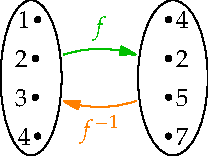
\includegraphics{inverse-easy}
	\end{minipage}
\end{example}


\begin{defn}{}{inversefn}
	A function $f:A\to B$ is \emph{invertible} if it has an \emph{inverse}: a function $f^{-1}:B\to A$ for which
	\[
		f^{-1}\bigl(f(x)\bigr)=x\quad\text{and}\quad f\bigl(f^{-1}(y)\bigr)=y \tag{$\ast$}
	\]
	for all possible inputs $x\in A$ and $y\in B$.
\end{defn}

Certainly Example \ref{ex:easyinvfunc} satisfies the input--output properties ($\ast$). Our concerns are identifying when a function is invertible, how to make it so if not, and how to compute an inverse. %To motivate this, we consider two simple examples.



\begin{examples}{}{invexs}
	%\exstart Define a simple function using a table or an arrow diagram
	% \begin{enumerate}\setcounter{enumi}{1}
	% \begin{minipage}[t]{0.74\linewidth}\vspace{-17pt}
	% \item[]\[\def\arraystretch{1.1}\begin{array}{c|cccc}
	% x&1&2&3&4\\\hline
	% f(x)&4&2&5&7
	% \end{array}\qquad\begin{array}{c|cccc}
	% y&4&2&5&7\\\hline
	% f^{-1}(y)&1&2&3&4
	% \end{array}
	% \]
	% Its inverse $f^{-1}$ is plainly the function obtained by \emph{reversing the arrows} or flipping the table upside-down. Certainly\vspace{-5pt}
	% \end{minipage}\hfill\begin{minipage}[t]{0.25\linewidth}\vspace{-17pt}
	% \flushright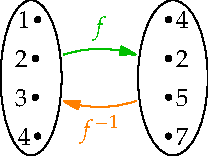
\includegraphics{inverse-easy}
	% \end{minipage}\par
	% \[f^{-1}\bigl(f(x)\bigr)=x\quad\text{and}\quad f\bigl(f^{-1}(y)\bigr)=y\tag{$\ast$}\]
	% for all possible inputs $x,y$ to either function, so inputs are indeed recovered from outputs.
	\exstart The function $f(x)=2x$ has inverse $f^{-1}(y)=\frac y2$.
	
	\begin{enumerate}\setcounter{enumi}{1}
		\begin{minipage}[t]{0.79\linewidth}\vspace{-10pt}
			\item[]The input--output conditions $(\ast)$ are certainly satisfied.
			\smallbreak
			The \textcolor{blue}{graph} admits an interpretation of $f^{-1}$ similar to the arrow diagram.
			\begin{itemize}\itemsep2pt
			  \item The function $f$ takes an input $x$, moves it \textcolor{Green}{vertically} to the graph, then \textcolor{Green}{projects} to the $y$-axis. This interpretation is precisely the vertical line test (Definition \ref{defn:function})!
			  \item The inverse function \emph{reverses the arrows}: transport an input $y$ \textcolor{orange}{horizontally} to the graph, then \textcolor{orange}{project} to the $x$-axis.
			\end{itemize}
		\end{minipage}
		\hfill
		\begin{minipage}[t]{0.2\linewidth}\vspace{-25pt}
			\flushright
			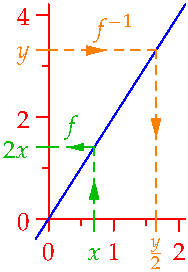
\includegraphics{inverses-line}
		\end{minipage}
		\smallbreak

		\begin{minipage}[t]{0.71\linewidth}\vspace{-5pt}
			\item\label{ex:invexs1} Consider $f(x)=x^2-1$. This time, when attempting to move a real number $y$ \textcolor{orange}{horizontally} to the graph, we usually encounter one of two problems:
			\begin{enumerate}\itemsep2pt
			  \item If $y>-1$, there are \textcolor{orange}{two choices} of $x$ (two intersections).
			  \item If $y<-1$, there is \textcolor{Purple}{no intersection} with the graph.
			\end{enumerate}
			The naïve approach of \emph{reversing the arrows} is insufficient to define an inverse. However, a simple remedy arises by staring at the graph:
			\begin{itemize}\itemsep2pt
			  \item Problem (a) goes away if we delete the \textcolor{Brown}{left half} of the graph. Equivalently, we \emph{restrict the domain} of $f$ to $[0,\infty)$. 
			  \item Problem (b) disappears if we insist that $y\ge-1$. Equivalently, we \emph{restrict the codomain} of $f$ to its \emph{range} $[-1,\infty)$. 
			\end{itemize}
		\end{minipage}
		\hfill
		\begin{minipage}[t]{0.28\linewidth}\vspace{0pt}
			\flushright
			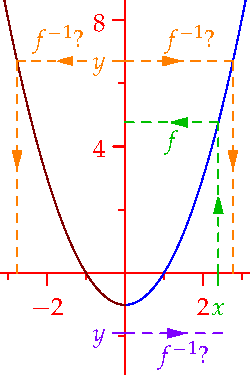
\includegraphics{inverses-quad}
		\end{minipage}
		\medbreak	
		After making these restrictions so that $f:[0,\infty)\to [-1,\infty)$, it is easily checked that
		\[
			f^{-1}(y)=\sqrt{y+1},\quad f^{-1}:[-1,\infty)\to[0,\infty)
		\]
		satisfies the input--output conditions $(\ast)$ and is therefore the inverse of $f$:
		\begin{gather*}
			x\in [0,\infty)\implies f^{-1}\bigl(f(x)\bigr) =\sqrt{(x^2-1)+1}=x\\
			y\in[-1,\infty)\implies f\bigl(f^{-1}(y)\bigr)=\bigl(\sqrt{y+1}\bigr)^2-1=y
		\end{gather*}
	\end{enumerate}
\end{examples}


\boldinline{What makes a function invertible?}

The fixes in the last example can be rephrased succinctly:
% \begin{quote}
\begin{center}
$\tcbhighmath{\text{
\emph{Horizontal line test}: every horizontal line must intersect the graph \emph{exactly once}}}$
\end{center}
% \end{quote}
This unpacks to two conditions, each of which addresses one of the problems seen in the example.

\begin{defn}{}{}
Let $f:A\to B$ be a function. We say that $f$ is:
\begin{enumeratea}
\item \emph{1--1/one-to-one} if distinct inputs $x_1\neq x_2\in A$ have distinct outputs $f(x_1)\neq f(x_2)$. Equivalently,
  \[
  	\text{Given $x_1,x_2\in A$, we have }\ f(x_1)=f(x_2)\Longrightarrow x_1=x_2
  \]
  If $A,B$ are sets of real numbers, each horizontal line intersects the graph \textcolor{orange}{at most once}.
  \item \emph{Onto} if $\operatorname{range}f=B$. Equivalently,
  \[
  	\text{Given $y\in B$, there is some $x\in A$ for which $y=f(x)$}
  \]
  If $A,B\subseteq\R$, the horizontal line through $y\in B$ intersects the graph \textcolor{Purple}{at least once}.
\end{enumeratea}
\end{defn}

Putting these ideas together, a function is both 1--1 and onto precisely when every $y\in B$ corresponds to a \emph{unique} $x\in A$ for which $y=f(x)$. In summary:

\begin{thm}{}{}
	$f:A\to B$ is invertible if and only if it is both 1--1 and onto. Its inverse is the function $f^{-1}:B\to A$ such that $f^{-1}(y)=x$ whenever $y=f(x)$.
\end{thm}

%Let us revisit our previous example in this context.

\begin{example*}{\ref*{ex:invexs}.\ref{ex:invexs1}, mk.\,II}{}
	Consider the two properties in the context of the example $f(x)=x^2-1$:
	\begin{enumeratea}
		\item $f(x_1)=f(x_2)\Longrightarrow x_1^2-1=x_2^2-1\Longrightarrow x_1^2=x_2^2\Longrightarrow x_1=\pm x_2$.\par
		To force $f$ to be 1--1, it is enough to \emph{restrict the domain} so that all $x$ have the same sign: the obvious choice is $\dom f=[0,\infty)$.
		\item $\operatorname{range} f=\bigl\{x^2-1:x\in[0,\infty)\bigr\}=[-1,\infty)$. We force $f$ to be onto by \emph{restricting its codomain} to $[-1,\infty)$.
	\end{enumeratea}
	The inverse function is obtained by solving $y=x^2-1$ for $x$:
	\[
		x^2=y+1\implies x=f^{-1}(y)=\sqrt{y+1}
	\]
	The \emph{non-negative square root} is used since $x\in\dom f=[0,\infty)$.
\end{example*}
\goodbreak


\boldinline{An algorithm for inverting functions}

Our discussion provides an algorithmic process for making a function $f:A\to B$ invertible and finding an inverse.
\begin{enumeratea}\itemsep2pt
	\item Check that $f$ is 1--1. If not, \emph{restrict the domain} until it is.
	\item Check that $f$ is onto. If not, \emph{redefine} $B=\operatorname{range} f$.
	\item Solve $y=f(x)$ for $x=f^{-1}(y)$.
\end{enumeratea}

Since $x$ is typically preferred as an input, it is common to \emph{switch} $x,y$ at the end of step 3 and write $y=f^{-1}(x)$. If $A,B\subseteq\R$, switching $x\leftrightarrow y$ is equivalent to \emph{reflecting the graph} in the line $y=x$.\smallbreak

Note also that step (a) likely involves a \emph{choice}; depending on how you restrict the domain, you can find multiple inverse functions! To see this in action, we return once more to our example.

\begin{example*}{\ref*{ex:invexs}.\ref{ex:invexs1}, mk.\,III}{}
	Recall that if $f(x)=x^2-1$, then
	\[
		f(x_1)=f(x_2)\implies x_1=\pm x_2
	\]
	Instead of restricting the domain to $[0,\infty)$, we can instead force $f$ to be 1--1 by taking the \textcolor{Brown}{other half} of the graph; by \emph{choosing} $\dom f=(-\infty,0]$. The range/codomain remains $[-1,\infty)$, but the inverse function is now different:
	\[
		x^2=y+1\implies x=-\sqrt{y+1}\in (-\infty,0]=\dom f \implies f^{-1}(x)=-\sqrt{x+1}
	\]
	This time the new domain for $f$ forced us to use the \emph{negative square root.}
	\begin{center}
		\begin{minipage}[t]{0.52\linewidth}\vspace{30pt}
			\centering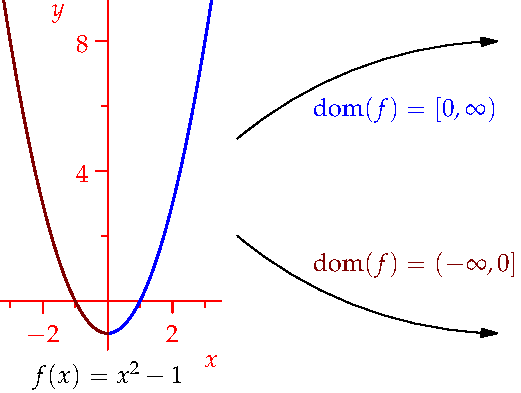
\includegraphics{inverses-combi}
		\end{minipage}
		\begin{minipage}[t]{0.35\linewidth}\vspace{0pt}
			\centering
			\begin{tabular}{@{}c@{}}
				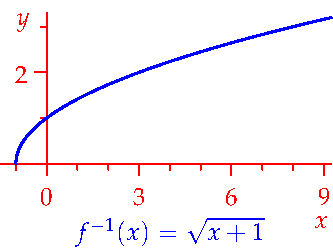
\includegraphics{inverses-combi2}\\[20pt]
				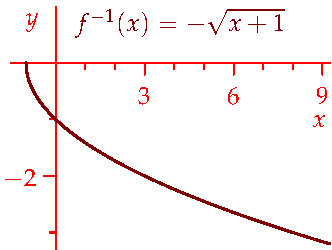
\includegraphics{inverses-combi3}
			\end{tabular}
		\end{minipage}
	\end{center}
	We could choose other domains on which $f$ is 1--1, but these are the most natural choices.
\end{example*}

The moral is that you cannot invert a function unless you are precise about its domain and range!

\goodbreak


\iffalse
\clearpage

\boldsubsubsection{OLD Version}

You've long been used to the idea of inverse functions: $g=f^{-1}$ means that $g$ takes the \emph{output} of $f$ and returns the \emph{input,} and vice versa.

\begin{defn}{}{inversefn}
Functions $f:A\to B$ and $g:B\to A$ are \emph{inverses} if two properties are satisfied:
\begin{itemize}
  \item Whenever $x\in A=\dom(f)$, we have $g\bigl(f(x)\bigr)=x$.
  \item Whenever $x\in B=\dom(g)$, we have $f\bigl(g(x)\bigr)=x$.
\end{itemize}
A function $f:A\to B$ is \emph{invertible} if it has an inverse function $g:B\to A$. 
\end{defn}

\begin{example}{}{}
The function $f(x)=2x$ has inverse $f^{-1}(x)=\frac 12x$.
\end{example}

The example shows the naïve way of approaching inverses. As is common in calculus/algebra, we defined functions using formulæ. Thankfully, if we follow standard conventions regarding the implied domain and codomain, then $f:\R\to\R$ and there is no problem with our example! Unfortunately, things are rarely so straightforward for almost any interesting function.

% \begin{example}{}{}
% Consider the formulæ $f(x)=x^2+2$ and $g(x)=\sqrt{x-2}$.
% \begin{enumerate}
%   \item Suppose $\dom(f)=A=\{1,2,3,4\}$ and $\operatorname{codom}(f)=B=\{3,6,11,18\}$.\par
% \begin{minipage}[t]{0.7\linewidth}\vspace{-5pt}
% It is easily checked that $g$ is the \emph{inverse function} to $f$, as is easily checked:
% \[g\bigl(f(x)\bigr)=\sqrt{(x^2+2)-2}=x,\quad f\bigl(g(x)\bigr)=\bigl(\sqrt{x-2}\bigr)^2+2=x\]
% All we are doing is reversing inputs and outputs. More formally, the domain and range/codomain switch over:
% \end{minipage}\hfill
% \begin{minipage}[t]{0.29\linewidth}\vspace{0pt}
% \hfill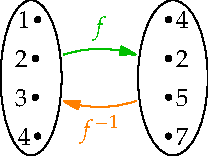
\includegraphics{inverse-easy}
% \end{minipage}\smallbreak
% \begin{gather*}
% A=\dom(f)=\operatorname{range}(g)=\operatorname{codom}(g)\\
% B=\dom(g)=\operatorname{range}(f)=\operatorname{codom}(f)
% \end{gather*}
% \end{enumerate}
% \end{example}


\begin{example}{}{inversex2}
Let $f(x)=x^2-1$ and $g(x)=\sqrt{x+1}$; intuitively these are inverse functions; indeed\par
\begin{minipage}[t]{0.7\linewidth}\vspace{-12pt}
\[f\bigl(g(3)\bigr)=f(2)=3\quad\text{and}\quad g\bigl(f(3)\bigr)=g(8)=3\]
In both cases, the second function returns the input of the first. However, replacing positives with negatives causes both calculations to fail:
\begin{enumeratea}
  \item When working with real numbers, $f\bigl(g(-3)\bigr)=f(\sqrt{-2})$ is meaningless and doesn't recover $-3$. This is a very silly thing to write, since $-2$ is not in the implied domain $\dom(g)=[-1,\infty)$.
  \item $g\bigl(f(-3)\bigr)=g(8)=3\neq -3$. The problem here is more subtle, arising from our unthinking use of the implied domain $\dom(f)=\R$:\vspace{-12pt}
\end{enumeratea}
  \[\textcolor{Green}{-3}\in\dom(f)=\R\ \text{ but }\ \textcolor{orange}{-3}\not\in\operatorname{range}(g)=[0,\infty)\]
Both cases illustrate the problem in using a formula to define a function: imprecision regarding \emph{domains} and \emph{ranges.}
\end{minipage}\hfill\begin{minipage}[t]{0.29\linewidth}\vspace{-5pt}
\flushright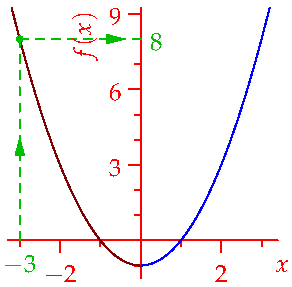
\includegraphics[scale=0.9]{inverses-poly3}\\
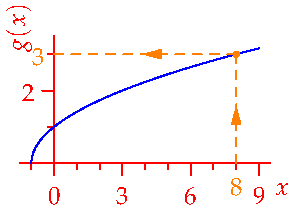
\includegraphics[scale=0.95]{inverses-poly2}
\end{minipage}\medbreak
The simple fix, disallow negative inputs to $f$, is implemented by \emph{restricting its domain} to $[0,\infty)$. The graph of $g$ is unchanged, but we've deleted the \textcolor{Brown}{left side} of the graph of $f$. We now have the inverse relationships we desire:
\begin{itemize}\itemsep0pt
  \item If $x\in\dom(f)=[0,\infty)$, then $g\bigl(f(x)\bigr)=\sqrt{(x^2-1)+1}=x$
  \item If $x\in\dom(g)=[-1,\infty)$, then $f\bigl(g(x)\bigr)=\bigl(\sqrt{x+1}\bigr)^2-1=x$
\end{itemize}
\end{example}




There is a lot going on here, though hopefully the simple fix of restricting the domain feels intuitive and low-tech. Our goal is to formalize and generalize this discussion. In particular, given a function $f:A\to B$, we have two questions: is $f$ invertible and, if so, how do we compute its inverse?

\goodbreak


\boldinline{What makes a function invertible?}

To motivate, we return to the example and consider how the \emph{vertical line test} (Definition \ref{defn:function}) provides an alternative viewpoint. A function may be envisioned as first transporting an input \emph{vertically} from the $x$-axis until it hits the graph, then projecting it \emph{horizontally} to the $y$-axis. An inverse function should reverse this process:\par

\begin{minipage}[t]{0.72\linewidth}\vspace{-3pt}
\begin{quote}
Transport an element on the $y$-axis \emph{horizontally} until it hits the graph, then project vertically onto the $x$-axis.
\end{quote}
The reason this process fails in our example is that we have \emph{two choices} for how to transport 9 horizontally to the graph:
\begin{itemize}\itemsep2pt
  \item The \textcolor{Green}{left-hand choice} produces $-3$ but does not correspond to $g$.
  \item The \textcolor{orange}{right-hand choice} recovers the correct original value $\textcolor{orange}{3}=g(8)$.
\end{itemize}
\end{minipage}\hfill\begin{minipage}[t]{0.27\linewidth}\vspace{-8pt}
\flushright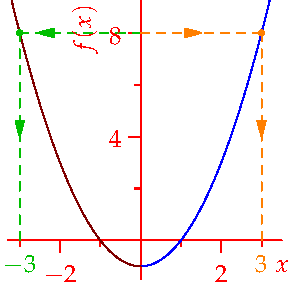
\includegraphics[scale=0.9]{inverses-poly1}
\end{minipage}\medbreak
The fix is to insist that $f$ passes a \emph{horizontal line test}: every such line should intersect the graph at most \emph{once}; this is exactly what we accomplish by restricting $\dom(f)=[0,\infty)$.\smallbreak
We get another useful observation for free. The inverse process (horizontal transport/vertical projection) is precisely what $g$ is doing once we switch the $x$ and $y$ axes: the \textcolor{blue}{graphs} of inverse functions are therefore related by \emph{reflection symmetry in the line $y=x$.}\smallbreak

Definition \ref{defn:inversefn} told us how to recognize an inverse function by its \emph{properties}. Our observation about reflections allows us to \emph{define} an inverse concretely for any function: when viewed as a set of ordered pairs $\bigl(a,f(a)\bigr)$, `reflection in the line $y=x$' simply means `reverse the order of each pair.'

\begin{defn}{}{}
Suppose $f:A\to B$ is a function. Its \emph{inverse} is the \emph{subset}
\[f^{-1}=\bigl\{(f(a),a):a\in A\bigr\}\subseteq B\times A\]
\end{defn}

The question of what makes a function invertible now becomes, `when is the \emph{set} $f^{-1}$ a function?' The answer to this is the vertical line test. Let's revisit our example.\par

\begin{example*}{\ref{ex:inversex2}, cont}{}
If $f(x)=x^2-1$ has domain $\R$, then its inverse is the set\par
\begin{minipage}[t]{0.65\linewidth}\vspace{-10pt}
\[f^{-1}=\bigl\{(y^2-1,y):y\in\R\bigr\}\]
obtained by reflecting the graph of $f$ in the line $y=x$. This is not a function because it fails the vertical line test in two ways:
\begin{enumerate}\itemsep2pt
  \item If \textcolor{magenta}{$x>-1$}, then the vertical line intersects the graph \emph{twice.}
  \item If \textcolor{cyan}{$x<-1$}, then the vertical line does not intersect the graph.
\end{enumerate}
Both issues have a simple fix:
\begin{enumerate}\itemsep2pt
  \item Restrict the \emph{domain} of $f$ to $A=[0,\infty)$.
  \item Restrict the \emph{codomain} of $f$ to $B=[-1,\infty)$.
\end{enumerate}
\end{minipage}\hfill\begin{minipage}[t]{0.34\linewidth}\vspace{-10pt}
\flushright\begin{tabular}{@{}c@{}}
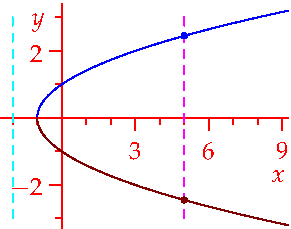
\includegraphics{inverses-poly4}\\
Graph of $f^{-1}$
\end{tabular}
\end{minipage}\medbreak
The inverse of the \textcolor{blue}{restricted} function $f:A\to B$ is now a \emph{function} $f^{-1}:B\to A$, $f(x)=\sqrt{x+1}$:
\[f^{-1}=\bigl\{(y^2-1,y):y\in[0,\infty)\bigr\} =\bigl\{(x,\sqrt{x+1}),x\in[-1,\infty)\bigr\}\]
\end{example*}


\goodbreak

It's time to put this all together and justify what should be a familiar algorithm. The vertical line test for the reflected graph of $f^{-1}$ becomes a \emph{horizontal line test} for the original function $f$.

\begin{thm}{Horizontal Line Test}{}
Let $f:A\to B$ be a function. Then $f$ is invertible if and only if it satisfies two conditions:
\begin{enumerate}
  \item (1--1/one-to-one)\lstsp Distinct inputs have distinct outputs:\footnotemark
  \[f(x_1)=f(x_2)\implies x_1=x_2\]
  This is equivalent to every \textcolor{magenta}{horizontal line} intersecting the graph \textcolor{magenta}{at most once}.
  \item (Onto)\lstsp Every potential output is realized; otherwise said $B=\operatorname{range}(f)$:
  \[\text{Given $y\in B$, there is some $x\in A$ for which $y=f(x)$}\]
  This is equivalent to a \textcolor{cyan}{horizontal line} through $y\in B$ intersecting the graph \textcolor{cyan}{at least once}.
\end{enumerate}
\end{thm}

\footnotetext{This means the same as $x_1\neq x_2\implies f(x_1)\neq f(x_2)$ but is easier to calculate with!}

Our original version of $f(x)=x^2-1$ failed both conditions when $f:\R\to\R$, but passes both when $f:[0,\infty)\to[-1,\infty)$.\smallbreak

The horizontal line test becomes three-step algorithm for finding inverse functions, of which the first two steps are the horizontal line test:
\begin{enumerate}
  \item Check that $f$ is 1--1. If not, \emph{restrict its domain} $A=\dom(f)$.
	\item \emph{Define} $B=\operatorname{range}(f)$.
	\item Switch $x,y$ and solve $x=f(y)\rightsquigarrow y=f^{-1}(x)$ in terms of $x$.
\end{enumerate}

When $f:A\to B$ is invertible, the construction makes clear why we must have
\[\dom(f^{-1})=B=\operatorname{range}(f),\quad \operatorname{range}(f^{-1})=\dom(f)\]

\begin{example*}{\ref{ex:inversex2}, cont}{}
The first step in our algorithm involves some \emph{choice.} If we instead restrict the domain so that $\dom(f)=(-\infty,0]$, then the function is still 1--1:
\begin{align*}
f(x_1)=f(x_2)&\implies x_1^2-1=x_2^2-1 \implies (x_1-x_2)(x_1+x_2)=0 \implies x_1=\pm x_2\\
&\implies x_1=x_2
\end{align*}
since both $x_1,x_2\le 0$ they cannot have opposite signs!\par
\begin{minipage}[t]{0.7\linewidth}\vspace{-5pt}
In the second step we still have $B=\operatorname{range}(f)=[-1,\infty)$. The result is \emph{another inverse,} as we may compute via step 3:
\begin{align*}
x=f(y)=y^2-1&\implies y^2=x+1\\
&\implies f^{-1}(x)=y=-\sqrt{x+1}
\end{align*}
\end{minipage}\hfill\begin{minipage}[t]{0.29\linewidth}\vspace{-30pt}
\flushright\begin{tabular}{@{}c@{}}
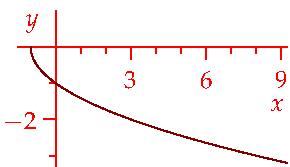
\includegraphics{inverses-poly5}\\
\textcolor{Brown}{$f^{-1}(x)=-\sqrt{x+1}$}
\end{tabular}
\end{minipage}\medbreak
where we chose the \emph{negative} square root since $\operatorname{range}(f^{-1})=\dom(f)=(-\infty,0]$. This, of course, is the result of reflecting the  \textcolor{Brown}{brown} half of the graph of $f$ across the line $y=x$.
\end{example*}

\goodbreak

\fi

We finish with an algebraically tougher example: you may feel that more detail is justified!

\begin{example}{}{function-easy}
	Let $y=f(x)=\frac 1{(x-2)^2}$. Its implied \textcolor{red}{\emph{domain}} consists of all real numbers except 2.
	\begin{description}
		\begin{minipage}[t]{0.68\linewidth}\vspace{-7pt}
			\item The \textcolor{Green}{\emph{vertical line test}} is clearly visible on the graph: every vertical line $x=a$, except $x=2$, intersects the graph exactly once.
			\item The \textcolor{Brown}{\emph{range}} is the interval $\R^+=(0,\infty)$ as can be seen by solving
			\[
				f(x)=y\iff \frac 1{x-2}=\pm \sqrt y\iff x=2\pm \frac 1{\sqrt y}
			\]
			Any positive output $y$ may be obtained via $y=f\bigl(2+\frac 1{\sqrt y}\bigr)$.\par
			The $\pm$-term shows that $f$ fails the \textcolor{orange}{\emph{horizontal line test}}: it isn't 1--1.
			\item There are two natural choices for an inverse:
			\begin{enumeratea}
			  \item Choose \textcolor{blue}{$\dom f=(2,\infty)$}, then $\pm\sqrt y=\frac 1{x-2}$ is \emph{positive}. We take the \emph{positive} square root and obtain the inverse function
			  \[
			  	g:(0,\infty)\to(2,\infty),\quad g(x)=2+\frac 1{\sqrt y}
			  \] 
			  \item Choose \textcolor{Purple}{$\dom f=(-\infty,2)$}, then $\pm\sqrt y=\frac 1{x-2}$ is \emph{negative} and we obtain a second inverse function
			  \[
			  	h:(0,\infty)\to(-\infty,2),\quad h(x)=2-\frac 1{\sqrt y}
			  \] 
			\end{enumeratea}
		\end{minipage}
		\hfill
		\begin{minipage}[t]{0.31\linewidth}\vspace{-12pt}
			\flushright
			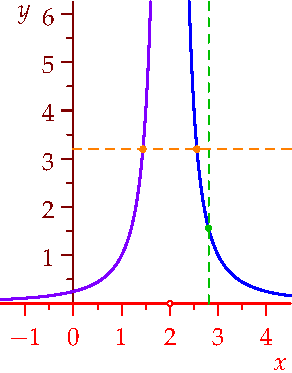
\includegraphics{functions-easyex1}\par
			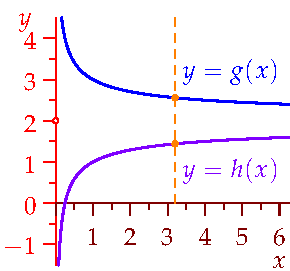
\includegraphics{functions-easyex2}
		\end{minipage}
	\end{description}
\end{example}



\begin{exercises}{}{}
	\exstart If $\dom f=\R$, check that $f(x)=x^3+8$ passes the horizontal line test. Find $f^{-1}$.
	
	\begin{enumerate}\setcounter{enumi}{1}
	  \item Consider $f(x)=x^2+2x-3$. Similarly to Example \ref{ex:invexs}, find \emph{two inverses} of $f$.
	  
	  \item Sketch the graph of the following function
	  \[
	  	f(x)=
	  	\begin{cases}
	  		x&\text{if }0\le x<1\\
	  		x-1&\text{if }1\le x<2\\
	  		x-2&\text{if }2\le x<3
	  	\end{cases}
	  \]
		Find \emph{three} domains on which $f$ is 1--1 and thus compute three distinct inverses.
	
	  \item Show that the following function $f:\R\to(\frac 32,\infty)$ is 1--1 and onto, sketch its graph and find $f^{-1}$. 
	  \[f(x)=\begin{cases}
	  3-\frac 12x&\text{if }x\le 2\\
	  2-\frac 1x&\text{if }x>2
	  \end{cases}\]
	  
	  \item (Hard)\lstsp Find the implied domain and range of $f(x)=\smash[b]{\frac{x+1}{1+\frac 1{x+1}}}$. Now find an interval on which $f$ is 1--1 and compute its inverse.
	  
	  \item An astute student observes that Definition \ref{defn:inversefn} only describes the properties satisfied by \emph{an} inverse and asks why we keep referring to \emph{the} inverse. How would you respond?
	  
	\end{enumerate}
\end{exercises}

\iffalse
\clearpage



\subsection{Increasing \& Decreasing Functions and Convexity}



Quadratic polynomials are a good excuse to introduce several related concepts.

\begin{defn}{}{}
Let $f:I\to\R$ be a function defined on an interval $I$. We say that $f$ is:
\begin{enumerate}
  \item \emph{Increasing} if $x_0<x_1\implies f(x_0)\le f(x_1)$.
% 	\item \emph{Strictly increasing} if the second inequality is strict; $f(x_1)<f(x_2)$.
	\item \emph{Convex (concave up)} if $x_0\neq x_1\implies (1-t)f(x_0)+tf(x_1)\ge f\bigl((1-t)x_0+tx_1\bigr)$ for all $0<t<1$. Otherwise said, the line segment joining any two points on the graph lies \emph{above} the graph.
\end{enumerate}
Reverse the inequalities to obtain the notions of \emph{decreasing} and \emph{concave down.} The inequalities can also be made strict to obtain \emph{strictly increasing} and \emph{strictly convex,} etc.
\end{defn}

\begin{minipage}[t]{0.45\linewidth}\vspace{0pt}
The function in the picture is convex where its graph is blue. If $0<t<1$, the  value
\[x_t=(1-t)x_1+tx_2\]
lies strictly between $x_1$ and $x_2$. At this point the function lies below the corresponding point on the line joining $(x_1,f(x_1))$ and $(x_2,f(x_2))$:
\[f(x_t)<(1-t)f(x_1)+tf(x_2)\]
\end{minipage}\begin{minipage}[t]{0.55\linewidth}\vspace{0pt}
\flushright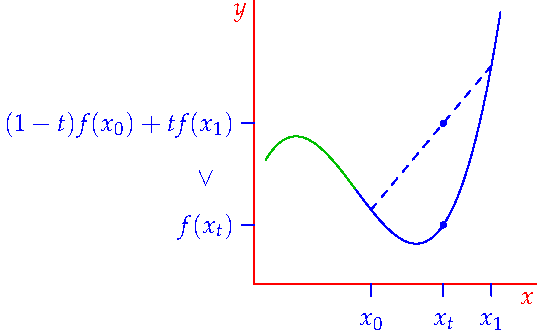
\includegraphics{poly-convex}
\end{minipage}\par

\begin{thm}{}{}
If $a>0$, then $f(x)=ax^2+bx+c$ is
\begin{enumerate}
  \item Increasing on the interval $[-\frac b{2a},\infty)$;
  \item Decreasing on the interval $(-\infty,-\frac b{2a}]$;
  \item Concave up on $\R$.
\end{enumerate}
The outcome is reversed if $a<0$.
\end{thm}

Instead of a formal argument, 
we consider the simplest example.

\begin{example}{}{}
$f(x)=x^2$ has apex $(0,0)$. Simply compare\par
\begin{minipage}[t]{0.65\linewidth}\vspace{0pt}
\[f(x_1)-f(x_0)=x_1^2-x_0^2 =(x_1-x_0)(x_1+x_0)\]
and consider two cases:
\begin{itemize}
  \item $0\le x_0<x_1\implies x_0+x_1>0\implies f(x_1)-f(x_0)>0$ so $f$ is \textcolor{blue}{strictly increasing}.
  \item $x_0<x_1\le 0\implies x_0+x_1<0\implies f(x_1)-f(x_0)<0$ so $f$ is \textcolor{Green}{strictly decreasing}.
\end{itemize}
Finally, for any $x_0,x_1\in\R$ and any $0<t<1$, a little algebra shows that
\end{minipage}\begin{minipage}[t]{0.35\linewidth}\vspace{-10pt}
\flushright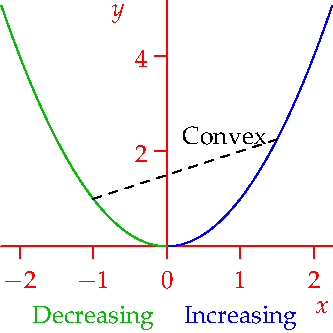
\includegraphics{poly-quad3}
\end{minipage}

\begin{align*}
f\bigl((1-t)x_0+tx_1\bigr)-(1-t)f(x_0)+tf(x_1)&=\bigl(x_0+t(x_1-x_0)\bigr)^2-(1-t)x_0^2+tx_1^2\\
&=t(t-1)\bigl(x_0+x_1\bigr)^2<0
\end{align*}
whence $f$ is convex (concave up). An alternative argument is in the exercises.
\end{example}



\begin{exercises}{}{}
\end{exercises}
\fi